\subsubsection{Checks of UE estimates with standard tracking }
As discussed in Section~\ref{sec:tracking}, the TPC had serious space-charge distortions during the 2013 p-Pb run. This resulted in a drastic drop in efficiency for tracking beyond 4 GeV. However, the TPC tracks can still be used for low $\pt$ tracking, which is the relevant region for underlying event measurements. 

Figure~\ref{fig:pPb_its_tpc_rho} shows the $\rho$ distribution measured with ITS-only and TPC+ITS tracks for photon-triggered events in p-Pb data. No significant difference is observed. To validate this the means of $\rho$ were found to be 3.129 GeV and 3.202 GeV for ITS and TPC+ITS $\rho$ values respectively. This rules out a large bias on the UE estimation due to larger fake rate for ITS tracking. This also constrains any impact on the poorer momentum resolution of the ITS tracking, which as shown in Section~\ref{sec:tracking} is about 10 times worse than for TPC+ITS tracks. This is expected because the UE-estimation is dominated by tracks with low momentum, and while the ITS tracking resolution is poorer, the smearing effects are relative minor. 

\begin{figure}
	\center
	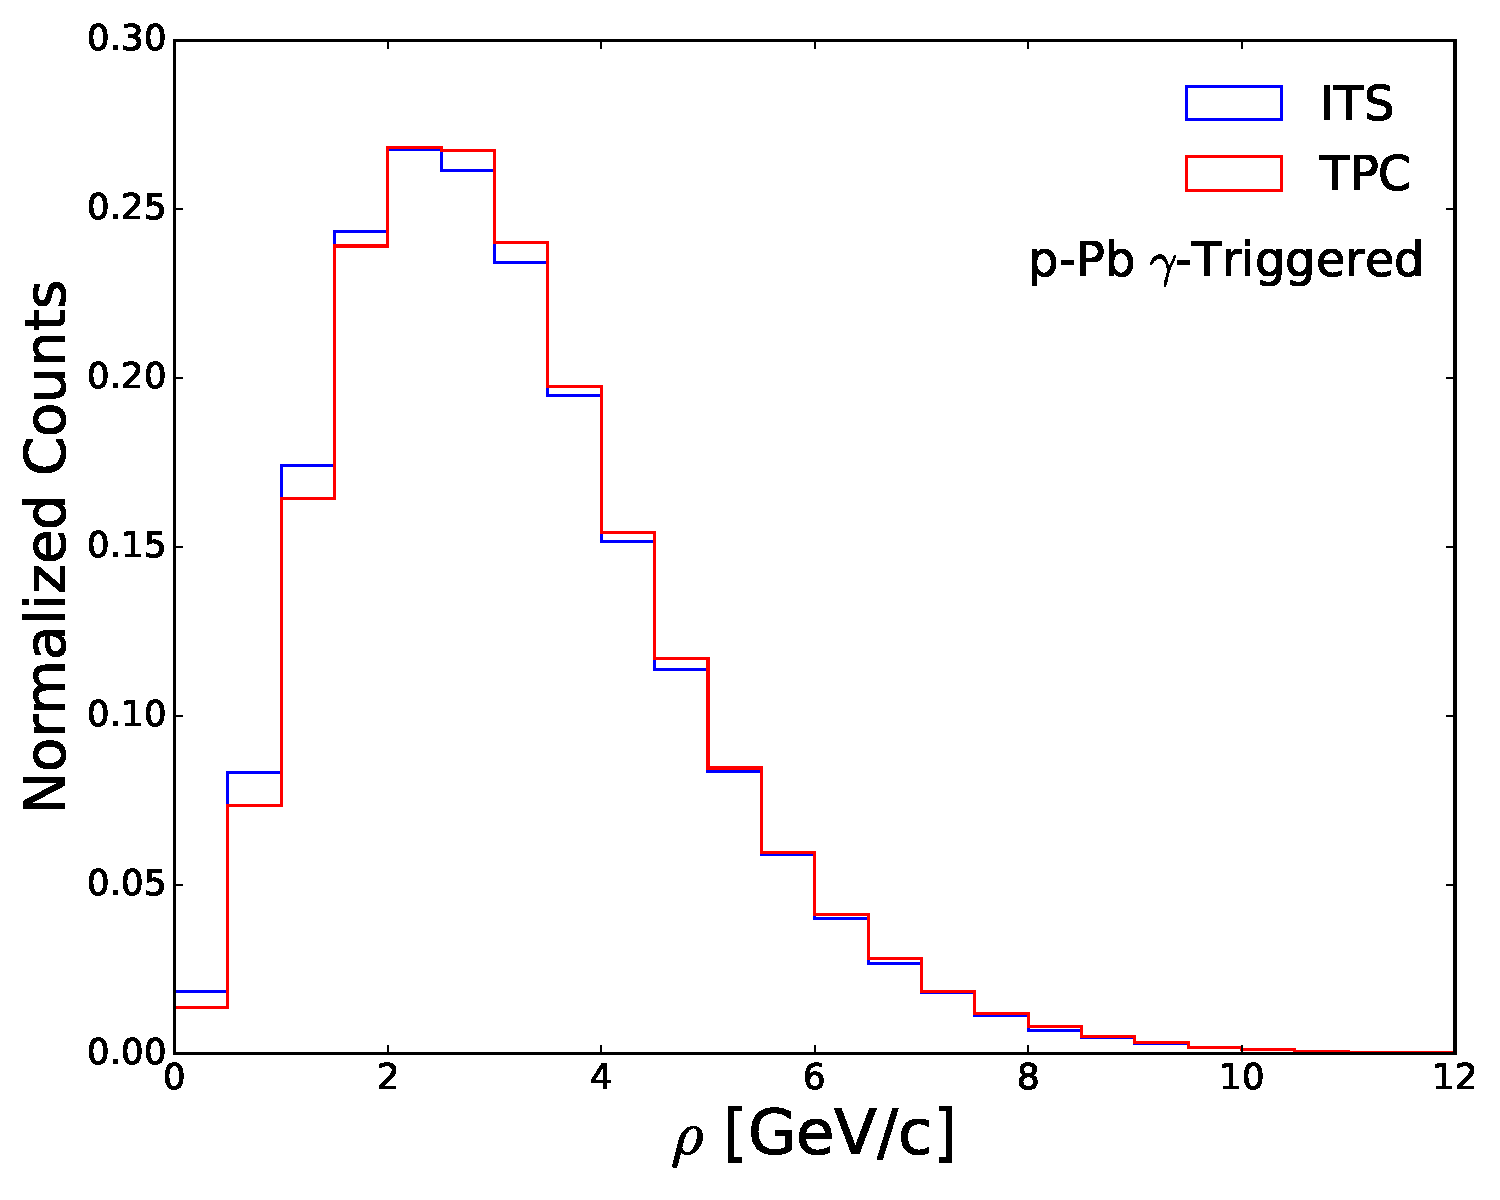
\includegraphics[width=0.5\textwidth]{JetReco/pPb_its_tpc_rho.pdf}
	\caption{A comparison between the median transverse momentum density distributions determined with ITS tracks (in blue) and TPC+ITS tracks (in red) in \pPb~photon-triggered data.}
	\label{fig:pPb_its_tpc_rho}
\end{figure}

\FloatBarrier
\subsubsection{Check for correlation between UE and hard-scale}
In this section we check that our UE-estimate is independent on the photon momentum required to be present in the event. Several studies have shown that above certain scale which is around few \GeVc, the UE density measured with $\rho$ and other observables reaches a plateau and only rises logarithmically with energy beyond that point. Thus, we can test our UE-estimation by changing the minimum $\pt$ that is required for an event. 

Figure~\ref{fig:ppandpPb_rho_thresholds} shows the $\rho$ distribution for photon-triggered events with different photon $\pt$ thresholds. No clear trend in the p-Pb distributions is observed. This is quantified in Table~\ref{tab:rhoestimatesCheck}, which shows the average $\rho$ for events that contain a photon with a minimum of 15, 20, 25, and 30 \GeVc  in pp and p-Pb data. The mean $\rho$ does not change within statistical uncertainties in the p-Pb case. A small but statistically significant trend is observed in the pp case.

\begin{figure}[h]
	\center
	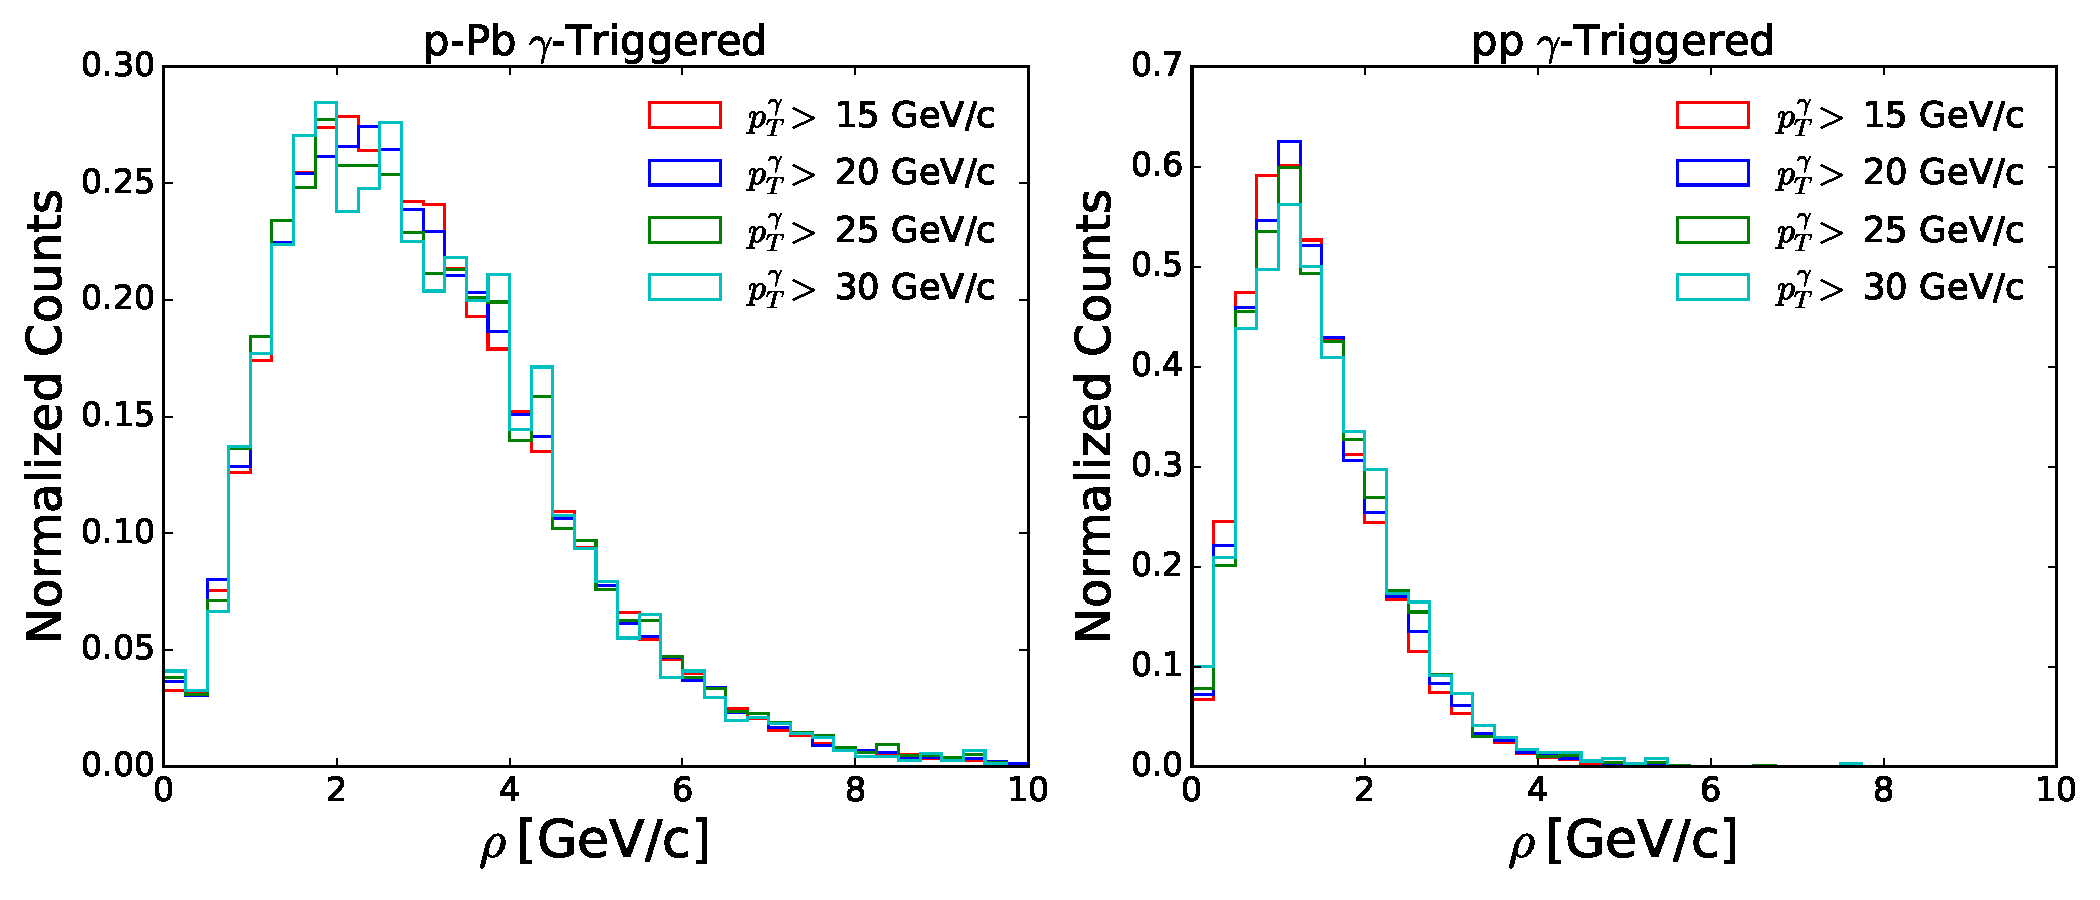
\includegraphics[width=1.0\textwidth]{JetReco/ppandpPb_rho.pdf}
	\caption{Median transverse momentum density distributions for events selected by a photon with different thresholds in photon-triggered events.}
	\label{fig:ppandpPb_rho_thresholds}
\end{figure}

\begin{table}[h]
   \centering
   \caption{Median transverse momentum density means in photon-triggered events for different photon momentum. The uncertainty quoted is statistical only.}
   \label{tab:rhoestimatesCheck}
   \begin{tabular*}{1.0\columnwidth}{@{\extracolsep{\fill}}lcc@{}}
    \hline
     &  p-Pb  & pp   \\
       \hline
$\langle\rho\rangle$ for $p_{\mathrm{T}}^{\gamma} >$ 15 \GeVc & 2.97 $\pm$ 0.01 & 1.40 $\pm$ 0.01  \\ 
              $\langle\rho\rangle$ for $p_{\mathrm{T}}^{\gamma}>$ 20 \GeVc & 2.97 $\pm$ 0.01& 1.43 $\pm$ 0.01\\ 
               $\langle\rho\rangle$ for $p_{\mathrm{T}}^{\gamma}>$ 25 \GeVc & 2.98 $\pm$ 0.02& 1.47 $\pm$ 0.02\\ 
               $\langle\rho\rangle$ for $p_{\mathrm{T}}^{\gamma}>$ 30 \GeVc  & 2.96 $\pm$ 0.03& 1.50  $\pm$ 0.02\\ 
              
           \hline        
   \end{tabular*}
\end{table}



%\subsection{New Figures}

%\begin{figure}
%    \centering
%    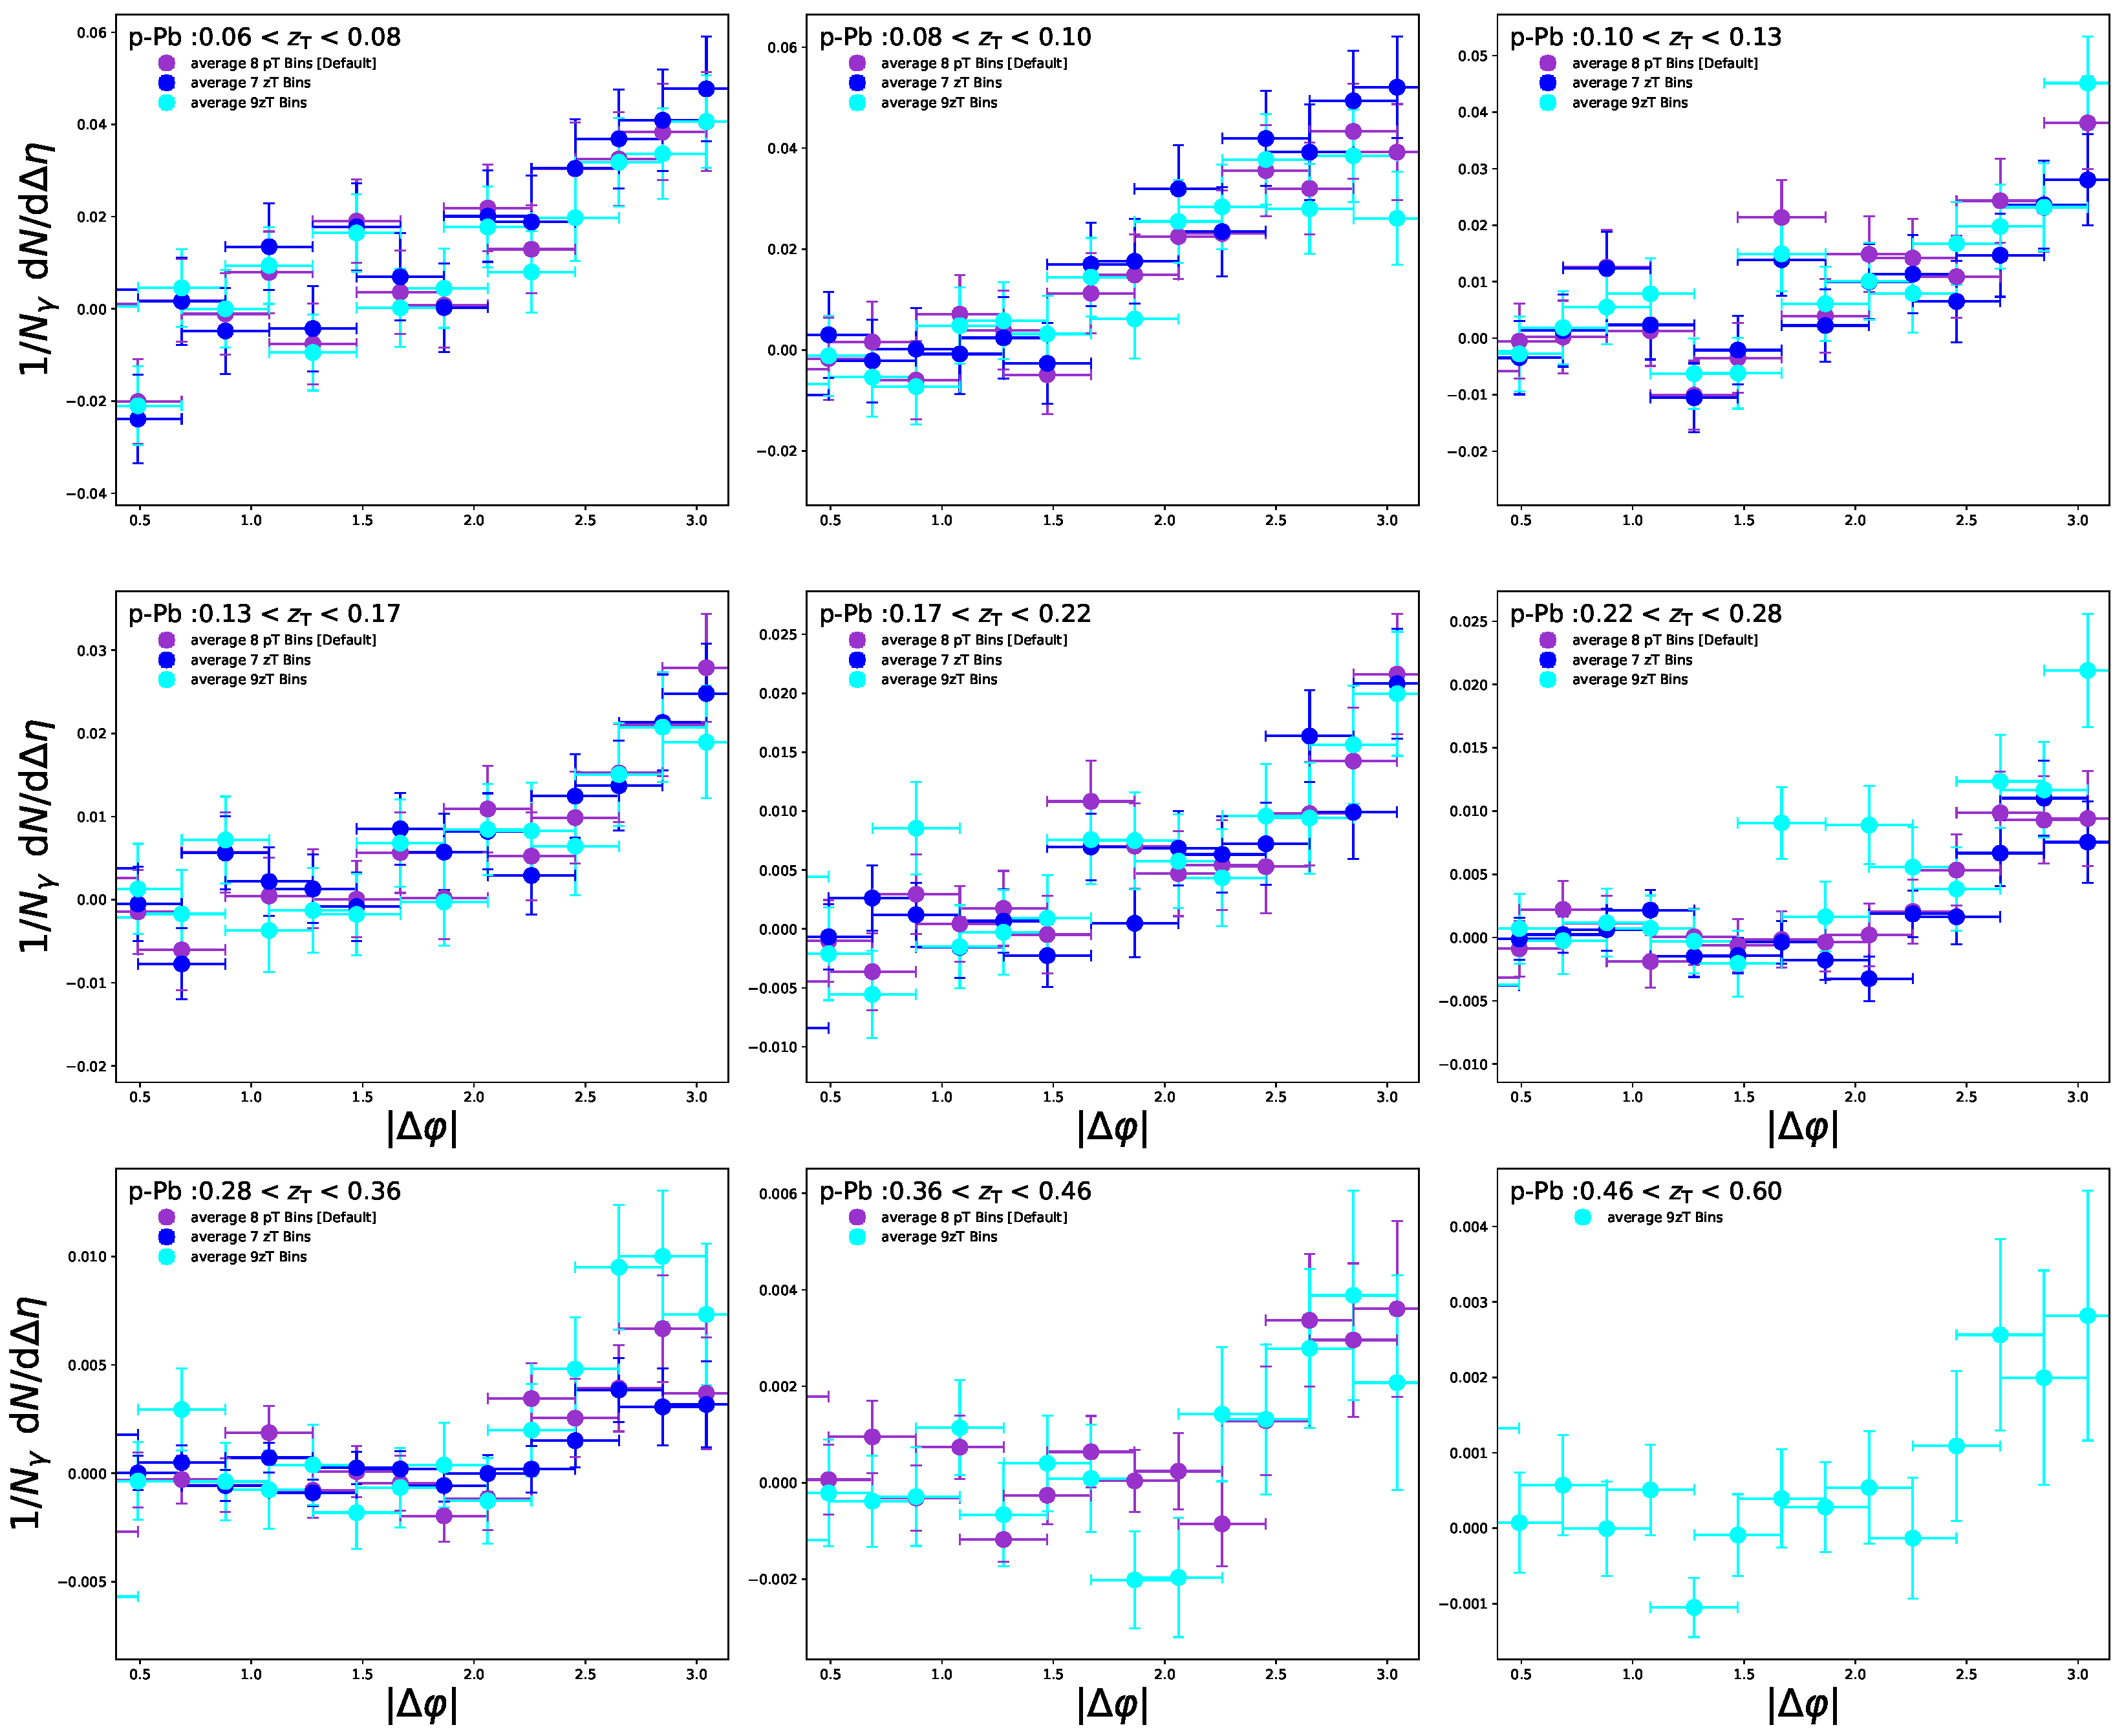
\includegraphics[width = 0.8\textwidth]{G-H_New/Cs_Averages_zT_Comparison.pdf}
%    \caption{Caption}
%\end{figure}{}


%\begin{figure}
%    \centering
%    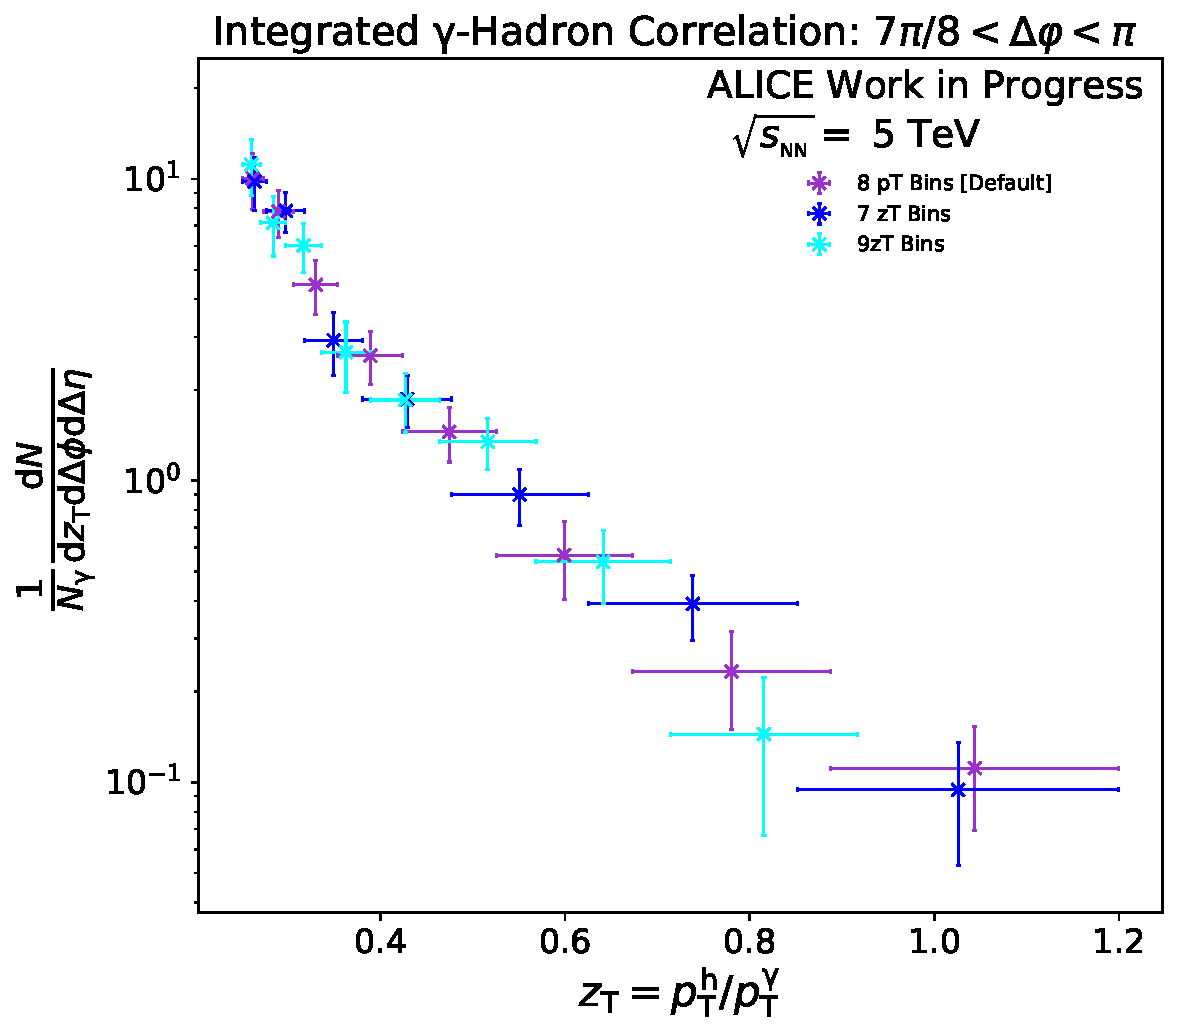
\includegraphics[width = 0.49 \textwidth] {G-H_New/FF_Averages_zT_Comparison.pdf}
%        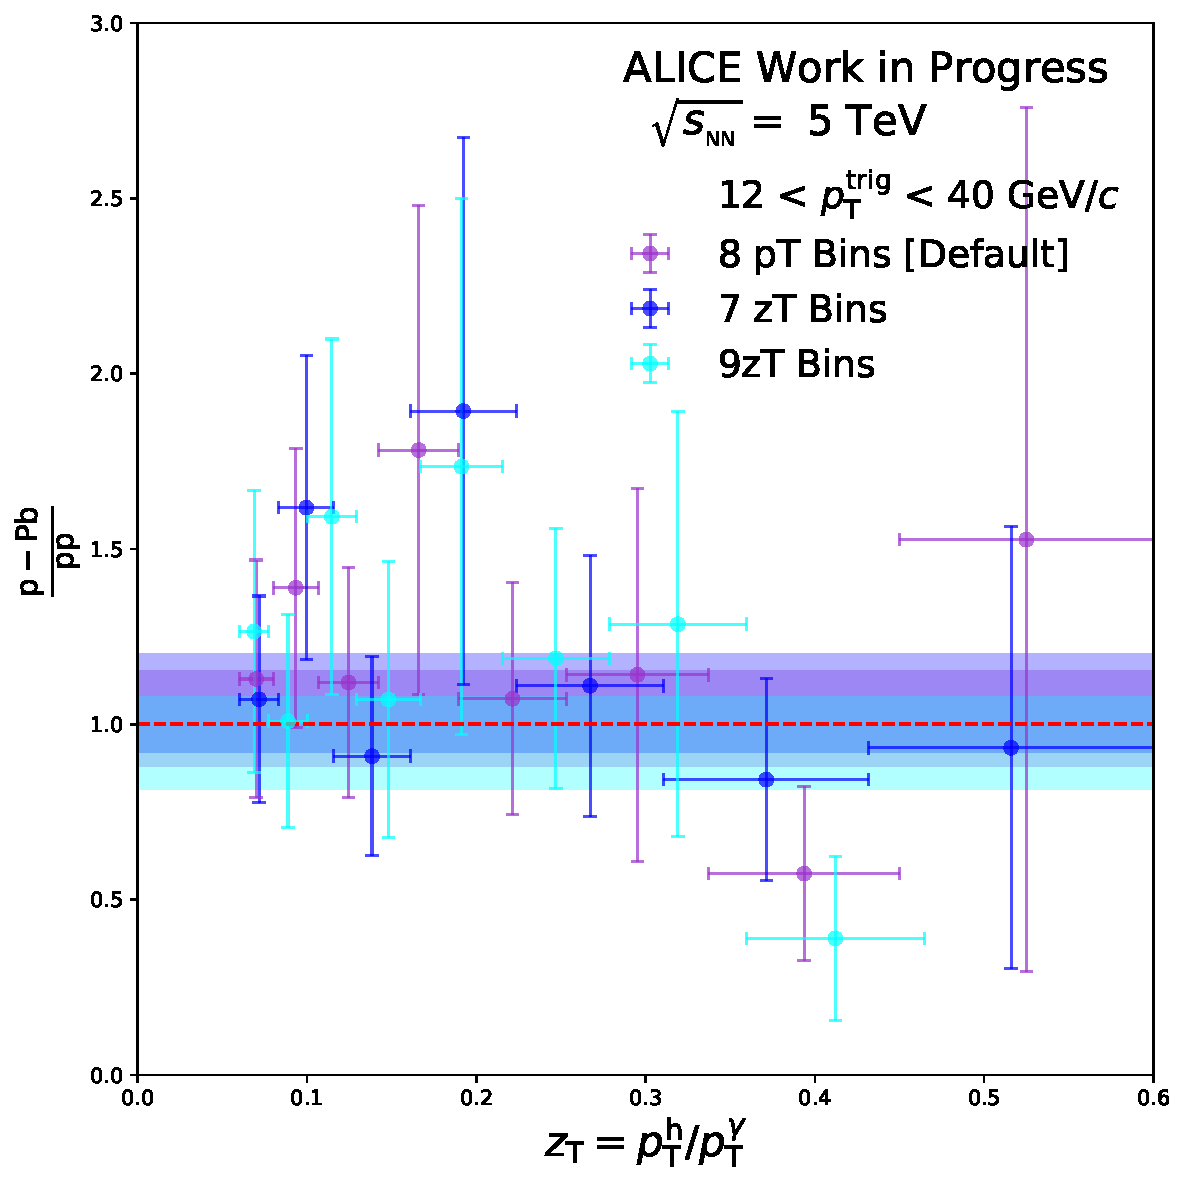
\includegraphics[width = 0.49\textwidth]{G-H_New/Ratio_FF_Averages_zT_Comparison.pdf}
%    \caption{Caption}
%\end{figure}{}




%\begin{figure}
%    \centering
%    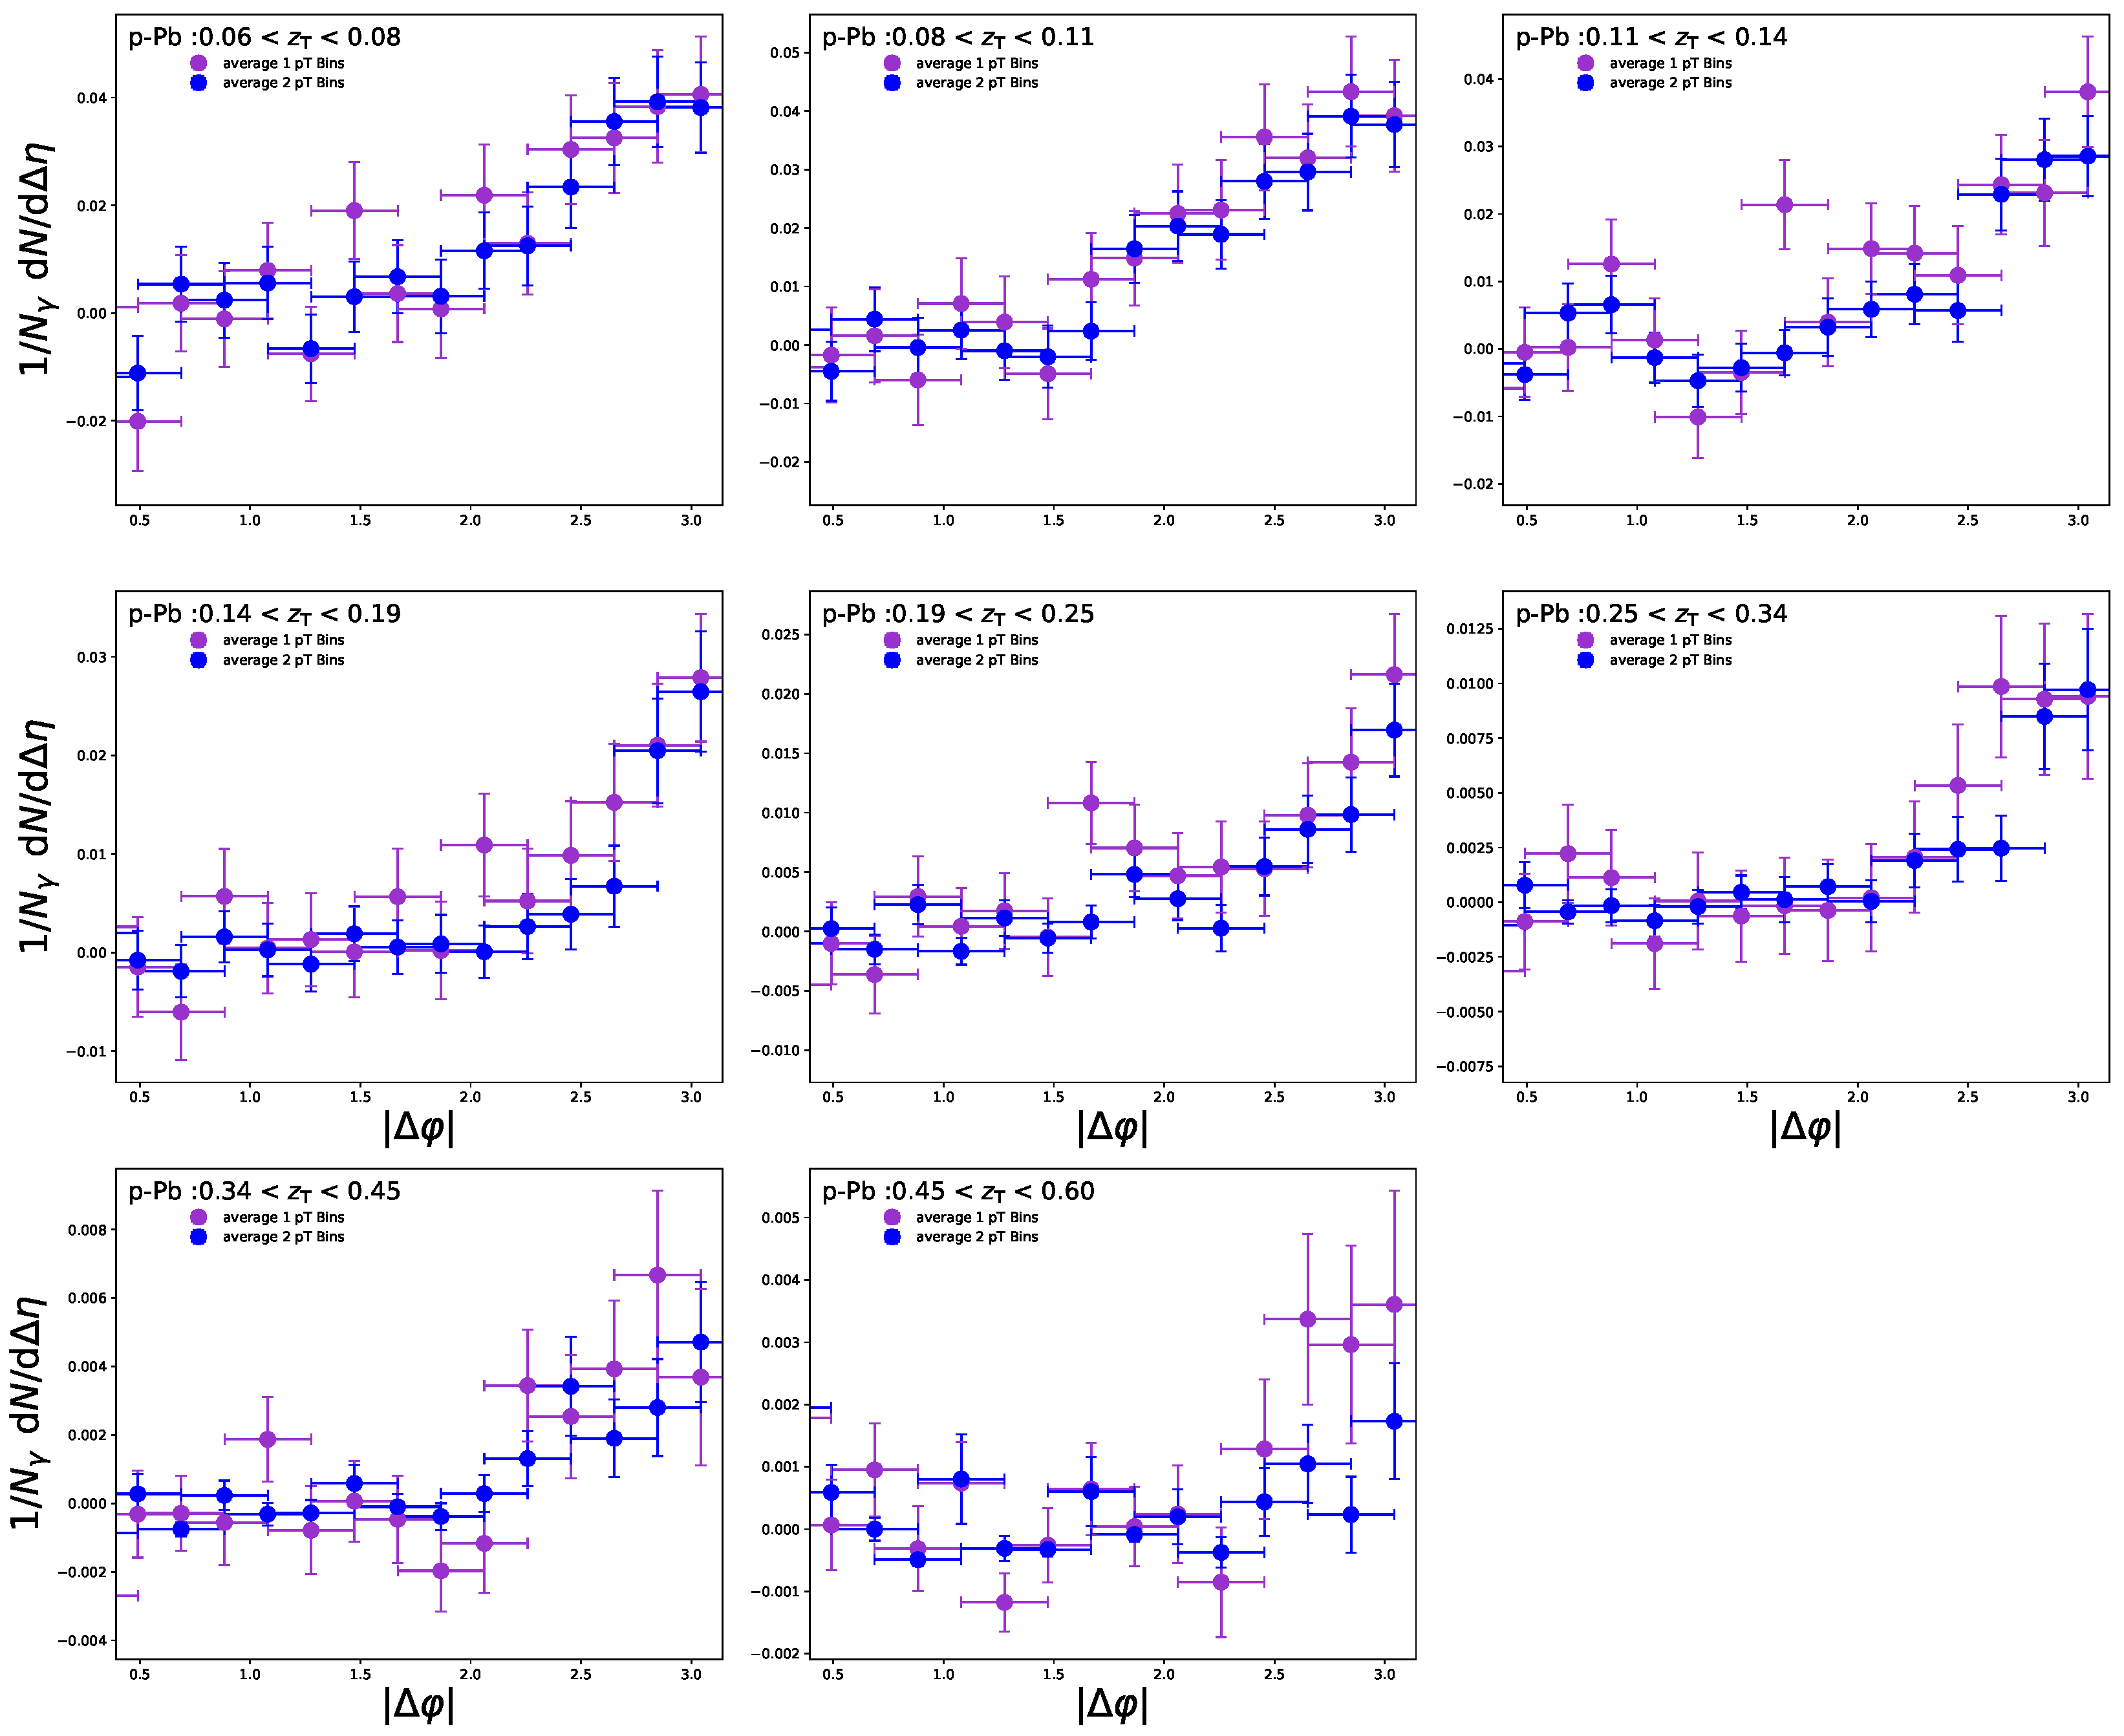
\includegraphics[width = 0.8\textwidth]{G-H_New/Cs_Averages_pT_Comparison.pdf}
%    \caption{Caption}
%\end{figure}{}


%\begin{figure}
%    \centering
%    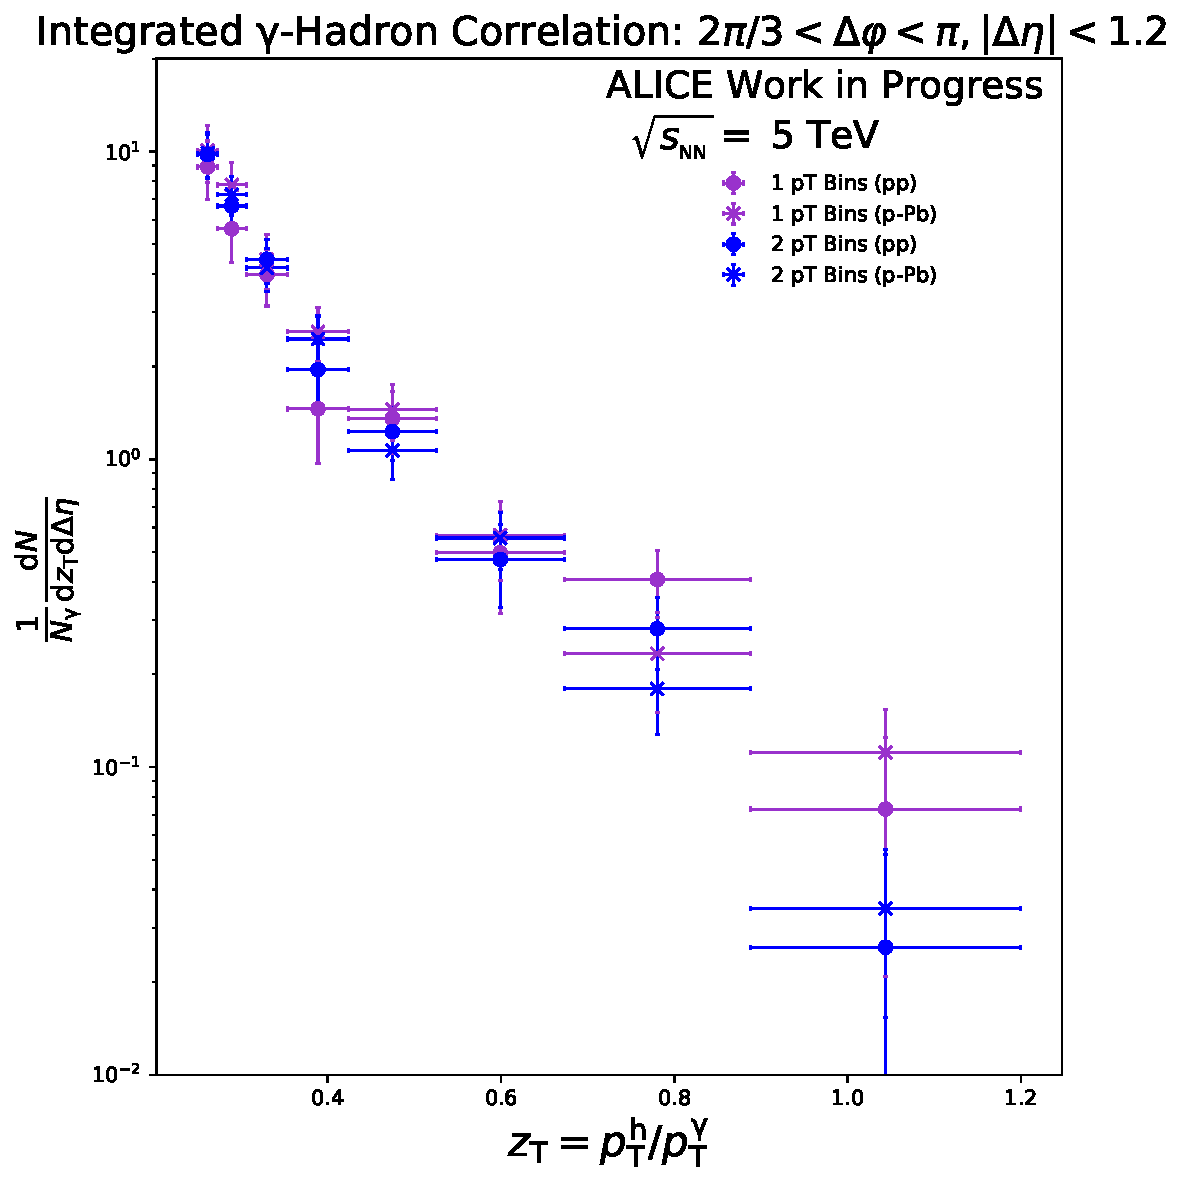
\includegraphics[width = 0.45 \textwidth]{G-H_New/FF_Averages_pT_Comparison.pdf}
%        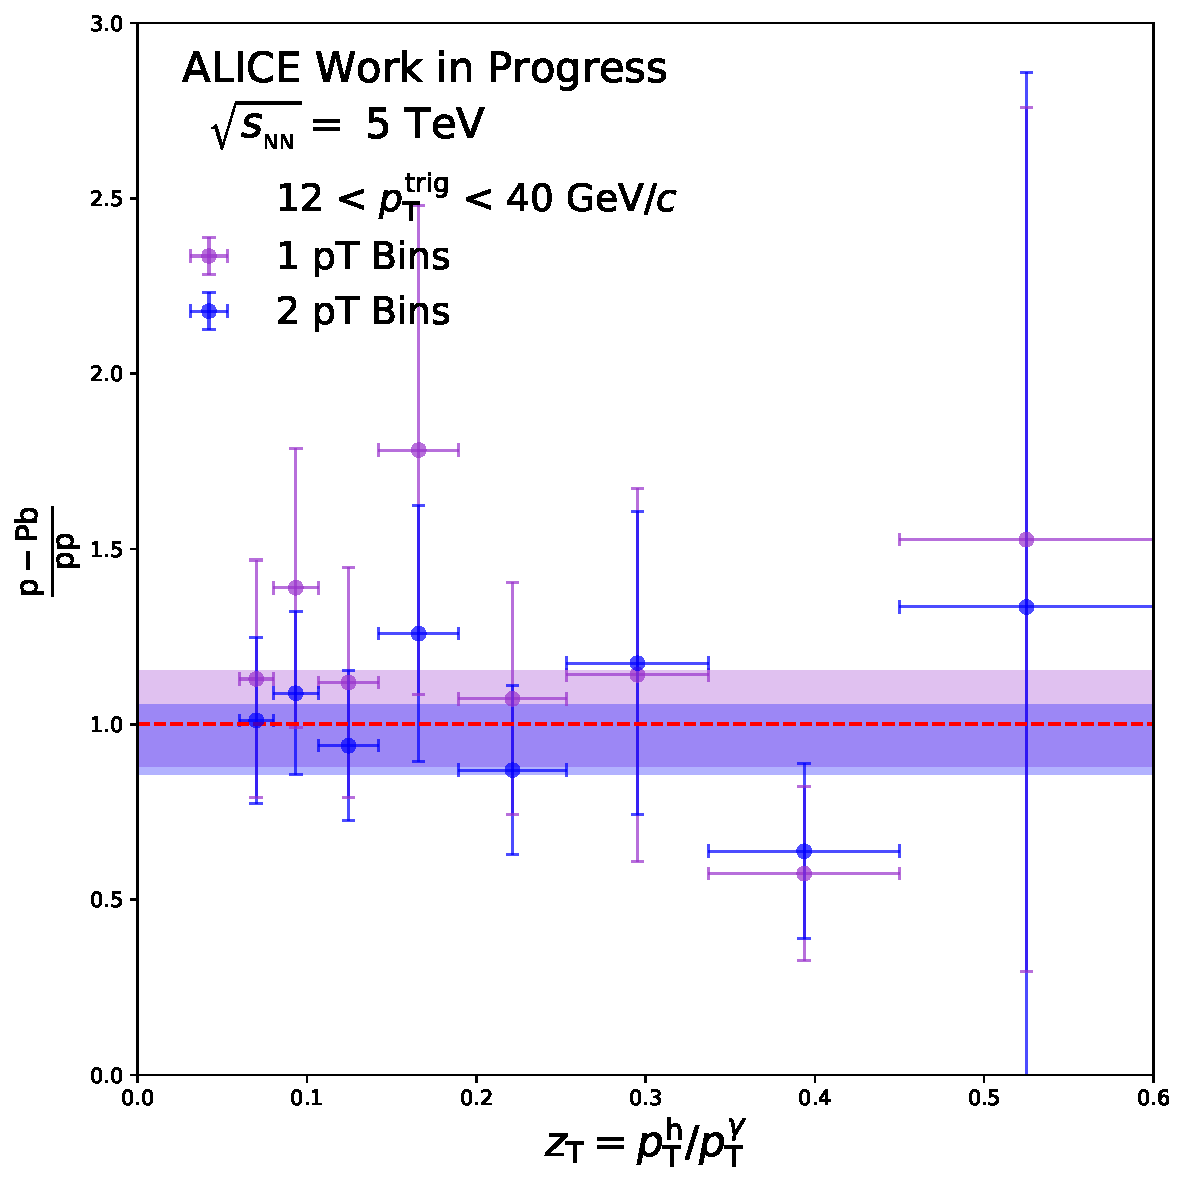
\includegraphics[width = 0.45\textwidth]{G-H_New/Ratio_FF_Averages_pT_Comparison.pdf}

 %   \caption{Caption}
 %   \label{fig:my_label}
%\end{figure}{}







%\begin{figure}
%\center
%\includegraphics[width=0.48\textwidth]{gammajet4}
%\caption{Angular separation between $\gammaiso$ and jets compared with Pythia}
%\end{figure}
%This measurement establishes a benchmark for photon identification and background estimation. 